% Mind Your Manners --- NeurIPS workshop carve.
%
% VENUE-NEUTRAL, like main.tex: the target workshop's .sty replaces the marked
% block below and nothing else changes. NeurIPS workshop page limits vary by
% workshop (4 pages is common, 8 at some); this carve is written to the 4-page
% body target, with references and the author block excluded as they usually are.
% Check the CFP before submitting and, if the limit is 8, the obvious additions
% are the per-turn regrade curve and the replication table from the full paper.
%
% The full 54-page manuscript is main.tex and remains the source of record; this
% document is a carve of it, not a replacement, and every number here is also in
% that one.
\documentclass[10pt]{article}

% ---------------- venue block: replace wholesale with e.g. \usepackage{neurips_2026} ----
\usepackage[letterpaper,margin=1in]{geometry}
\usepackage[T1]{fontenc}
\usepackage[utf8]{inputenc}
\usepackage{lmodern}
% ---------------------------------------------------------------------------------------

\usepackage{amsmath,amssymb}
\usepackage{booktabs,array}
\usepackage{graphicx}
\graphicspath{{figures/}}
\usepackage{caption}
\usepackage[hidelinks]{hyperref}
\usepackage[numbers,sort&compress]{natbib}
\usepackage{microtype}
\usepackage{enumitem}
\usepackage{textcomp}

% Same 21 declarations as main.tex: pdflatex, not a Unicode engine, because
% lualatex could not resolve Latin Modern in the build environment.
\DeclareUnicodeCharacter{2014}{---}
\DeclareUnicodeCharacter{2013}{--}
\DeclareUnicodeCharacter{00A7}{\S}
\DeclareUnicodeCharacter{2212}{\ensuremath{-}}
\DeclareUnicodeCharacter{00D7}{\ensuremath{\times}}
\DeclareUnicodeCharacter{0394}{\ensuremath{\Delta}}
\DeclareUnicodeCharacter{00B1}{\ensuremath{\pm}}
\DeclareUnicodeCharacter{26A0}{\textbf{[!]}}
\DeclareUnicodeCharacter{2026}{\ldots}
\DeclareUnicodeCharacter{2248}{\ensuremath{\approx}}
\DeclareUnicodeCharacter{2265}{\ensuremath{\geq}}
\DeclareUnicodeCharacter{00B7}{\ensuremath{\cdot}}
\DeclareUnicodeCharacter{00B2}{\ensuremath{^2}}
\DeclareUnicodeCharacter{00E8}{\`e}
\DeclareUnicodeCharacter{03C7}{\ensuremath{\chi}}
\DeclareUnicodeCharacter{03B1}{\ensuremath{\alpha}}
\DeclareUnicodeCharacter{2080}{\ensuremath{_0}}
\DeclareUnicodeCharacter{2085}{\ensuremath{_5}}
\DeclareUnicodeCharacter{2087}{\ensuremath{_7}}
\DeclareUnicodeCharacter{2088}{\ensuremath{_8}}
\DeclareUnicodeCharacter{2089}{\ensuremath{_9}}

\usepackage{calc}
\providecommand{\real}[1]{#1}
\providecommand{\tightlist}{}
\providecommand{\pandocbounded}[1]{#1}

% The source headings carry their own numbering, as in the full paper.
\setcounter{secnumdepth}{0}
\setlist{nosep,leftmargin=1.4em}
\captionsetup{font=small,labelfont=bf}
\setlength{\emergencystretch}{3em}
\sloppy

\title{\textbf{Mind your manners? Demand, not register,\\is what moves an LLM agent}}
\author{%
  % TODO: author block --- name, affiliation, contact. Deliberately last.
  \textit{[author name withheld for review]}\\
  \textit{Independent researcher}
}
\date{}

\begin{document}
\maketitle

\input{workshop-sections/00-front}
\input{workshop-sections/01-demand}

\begin{figure}[t]
  \centering
  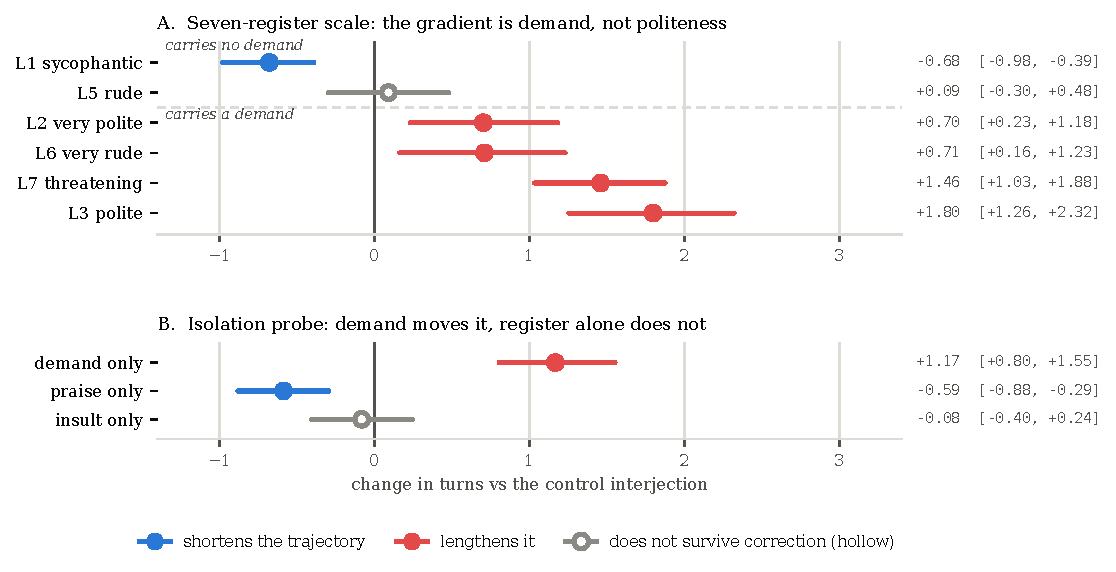
\includegraphics[width=\linewidth]{demand-vs-register.pdf}
  \caption{\textbf{Demand, not register, orders the effect.}
    Change in acting turns against the control interjection, with 95\% clustered
    intervals. \textbf{A}: the four demand-carrying arms do not overlap the two
    that carry none, and register does not sort them -- each side holds one
    flattering and one hostile arm. \textbf{B}: the isolation probe, where demand
    and affect are varied separately. Hollow markers do not survive
    Benjamini--Hochberg correction.}
  \label{fig:demand-vs-register}
\end{figure}

\input{workshop-sections/02-closing}

\begin{figure}[t]
  \centering
  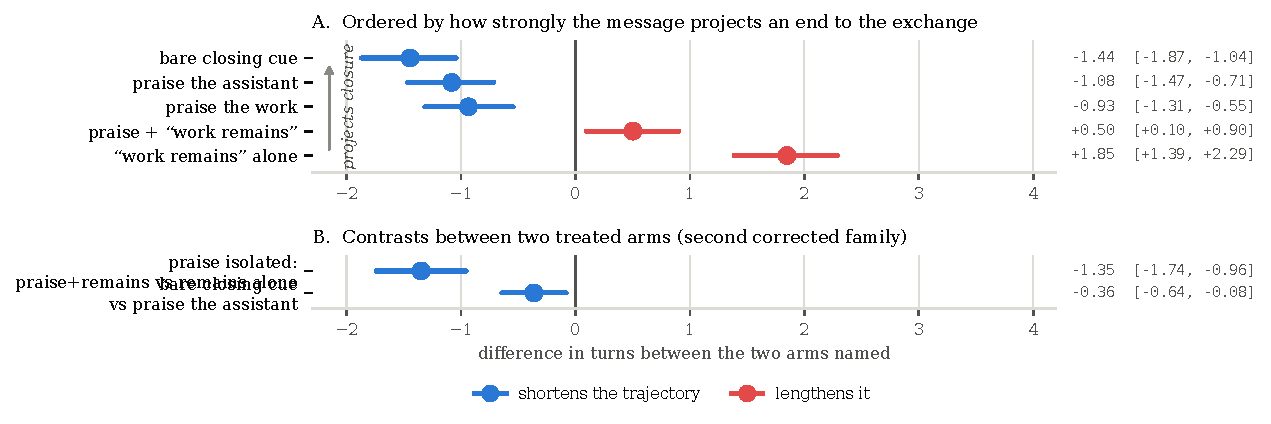
\includegraphics[width=\linewidth]{closing-cue.pdf}
  \caption{\textbf{Closing cues curtail the agent.}
    \textbf{A}: six arms ordered by how strongly the message projects an end to
    the exchange. The ordering is monotone, and the bare closing cue -- which
    praises nothing, evaluates nothing and claims nothing about task state --
    produces the largest reduction in the study. \textbf{B}: the two
    within-design contrasts, which compare one treated arm against another
    rather than against control.}
  \label{fig:closing-cue}
\end{figure}

\input{workshop-sections/03-close}

\bibliographystyle{plainnat}
\bibliography{references}

\end{document}
